\documentclass[compress]{beamer}

\usepackage[czech]{babel}
\usepackage{appendixnumberbeamer}

\usetheme{Madrid}
\useoutertheme{miniframes} % Alternatively: miniframes, infolines, split
\useinnertheme{circles}

%\setbeamertemplate{background} 
%{
%	
\includegraphics[width=0.8\textwidth]{img/background-kiv.pdf}
%}

%\definecolor{UBCblue}{rgb}{0.04706, 0.13725, 0.26667} % UBC Blue (primary)
\definecolor{UBCblue}{rgb}{0.04706, 0.13725, 0.26667} % UBC Blue (primary)
\definecolor{UBCgrey}{rgb}{0.3686, 0.5255, 0.6235} % UBC Grey (secondary)

\setbeamercolor{palette primary}{bg=UBCblue,fg=white}
\setbeamercolor{palette secondary}{bg=UBCblue,fg=white}
\setbeamercolor{palette tertiary}{bg=UBCblue,fg=white}
\setbeamercolor{palette quaternary}{bg=UBCblue,fg=white}
\setbeamercolor{structure}{fg=UBCblue} % itemize, enumerate, etc
\setbeamercolor{section in toc}{fg=UBCblue} % TOC sections

\setbeamertemplate{background} 
{
	
\includegraphics[width=\paperwidth,height=\paperheight]{img/background.png}
}

% Override palette coloring with secondary
\setbeamercolor{subsection in head/foot}{bg=UBCgrey,fg=white}
\setbeamertemplate{caption}[numbered]
\setbeamercovered{transparent}

\usepackage{xcolor}
\usepackage{fontspec}
\usefonttheme{serif}

\title[Rpi Zero emulátor]{Emulátor ARMv6 procesoru \\ pro emulaci prostředí Raspberry Pi}
\date{17. 06. 2024}
\author[Bc. Jakub Šilhavý]{Bc. Jakub Šilhavý}
\institute[KIV ZČU]{vedoucí práce: Ing. Martin Úbl \\ \bigskip Katedra informatiky a výpočetní techniky \\ Fakulta aplikovaných věd \\ Západočeská univerzita v Plzni}

\begin{document}
	
\begin{frame}
    \titlepage
\end{frame}

\section{Zadání práce}

\subsection{Zadání \& cíl práce}

\begin{frame}
	\begin{block}{Cíl práce}
		\begin{itemize}
			\item návrh a implementace emulátoru platformy \textbf{Raspberry Pi Zero}
			\begin{itemize}
				\item emulace instrukcí procesoru \texttt{ARM1176JZF-S} (\texttt{ARMv6})
				\item emulace základních periferií \texttt{µC} \texttt{BCM2835} (\texttt{GPIO}, \texttt{Mini\_UART}, \texttt{BSC}, ...)
			\end{itemize}
		\end{itemize}
	\end{block}
	\begin{columns}
		\column{0.57\textwidth}
		\begin{enumerate}
			\item vzdělávací účely
			\begin{itemize}
				\item vizualizace principů \texttt{OS}
				\item embedded vývoj
			\end{itemize}
			\item testování a ladění \texttt{SW}
			\item prototypování \texttt{HW}
			\begin{itemize}
				\item připojení externích periferií
				\item návrh vlastního systému
			\end{itemize}
		\end{enumerate}
		\column{0.4\textwidth}
		\begin{figure}
			\centering
			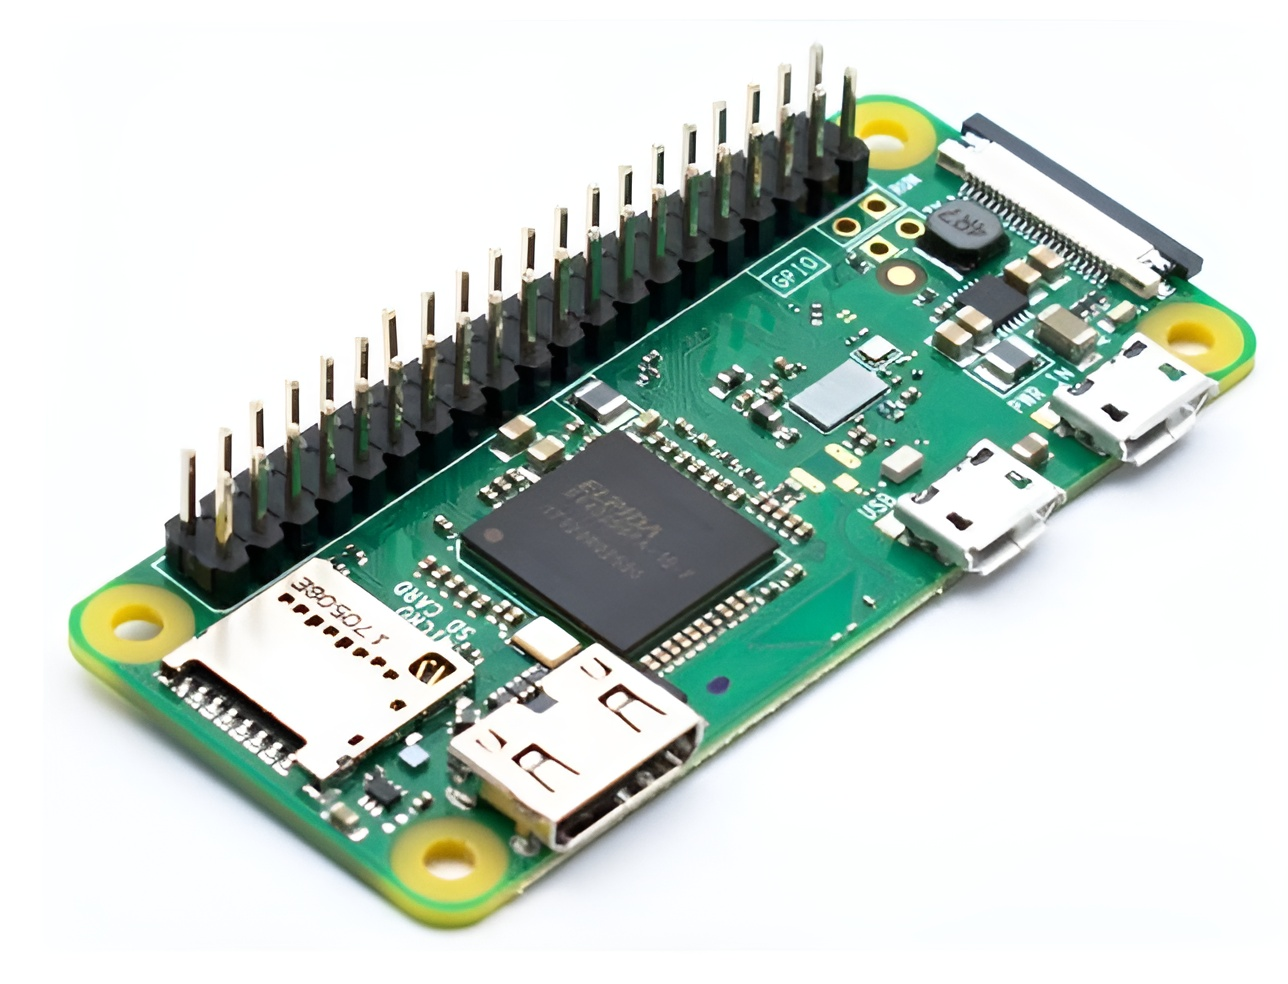
\includegraphics[width=0.60\textwidth]{img/rpi_zero.jpeg}
			\caption{Raspberry Pi Zero}
			\label{Raspberry Pi Zero}
		\end{figure}
	\end{columns}
	\vspace{0.2cm}
	\noindent\makebox[\linewidth]{\rule{\textwidth}{0.4pt}}
	\vspace{-0.4cm}
	\begin{itemize}
		\item použití \href{https://github.com/MartinUbl/KIV-RTOS}{\beamergotobutton{KIV-RTOS}} pro ověření správnosti výsledného emulátoru
	\end{itemize}
\end{frame}

\subsection{\texttt{ARM} procesory a jejich aplikace}

\begin{frame}
	\begin{columns}
		\column{0.45\textwidth}
			\begin{figure}
			\centering
			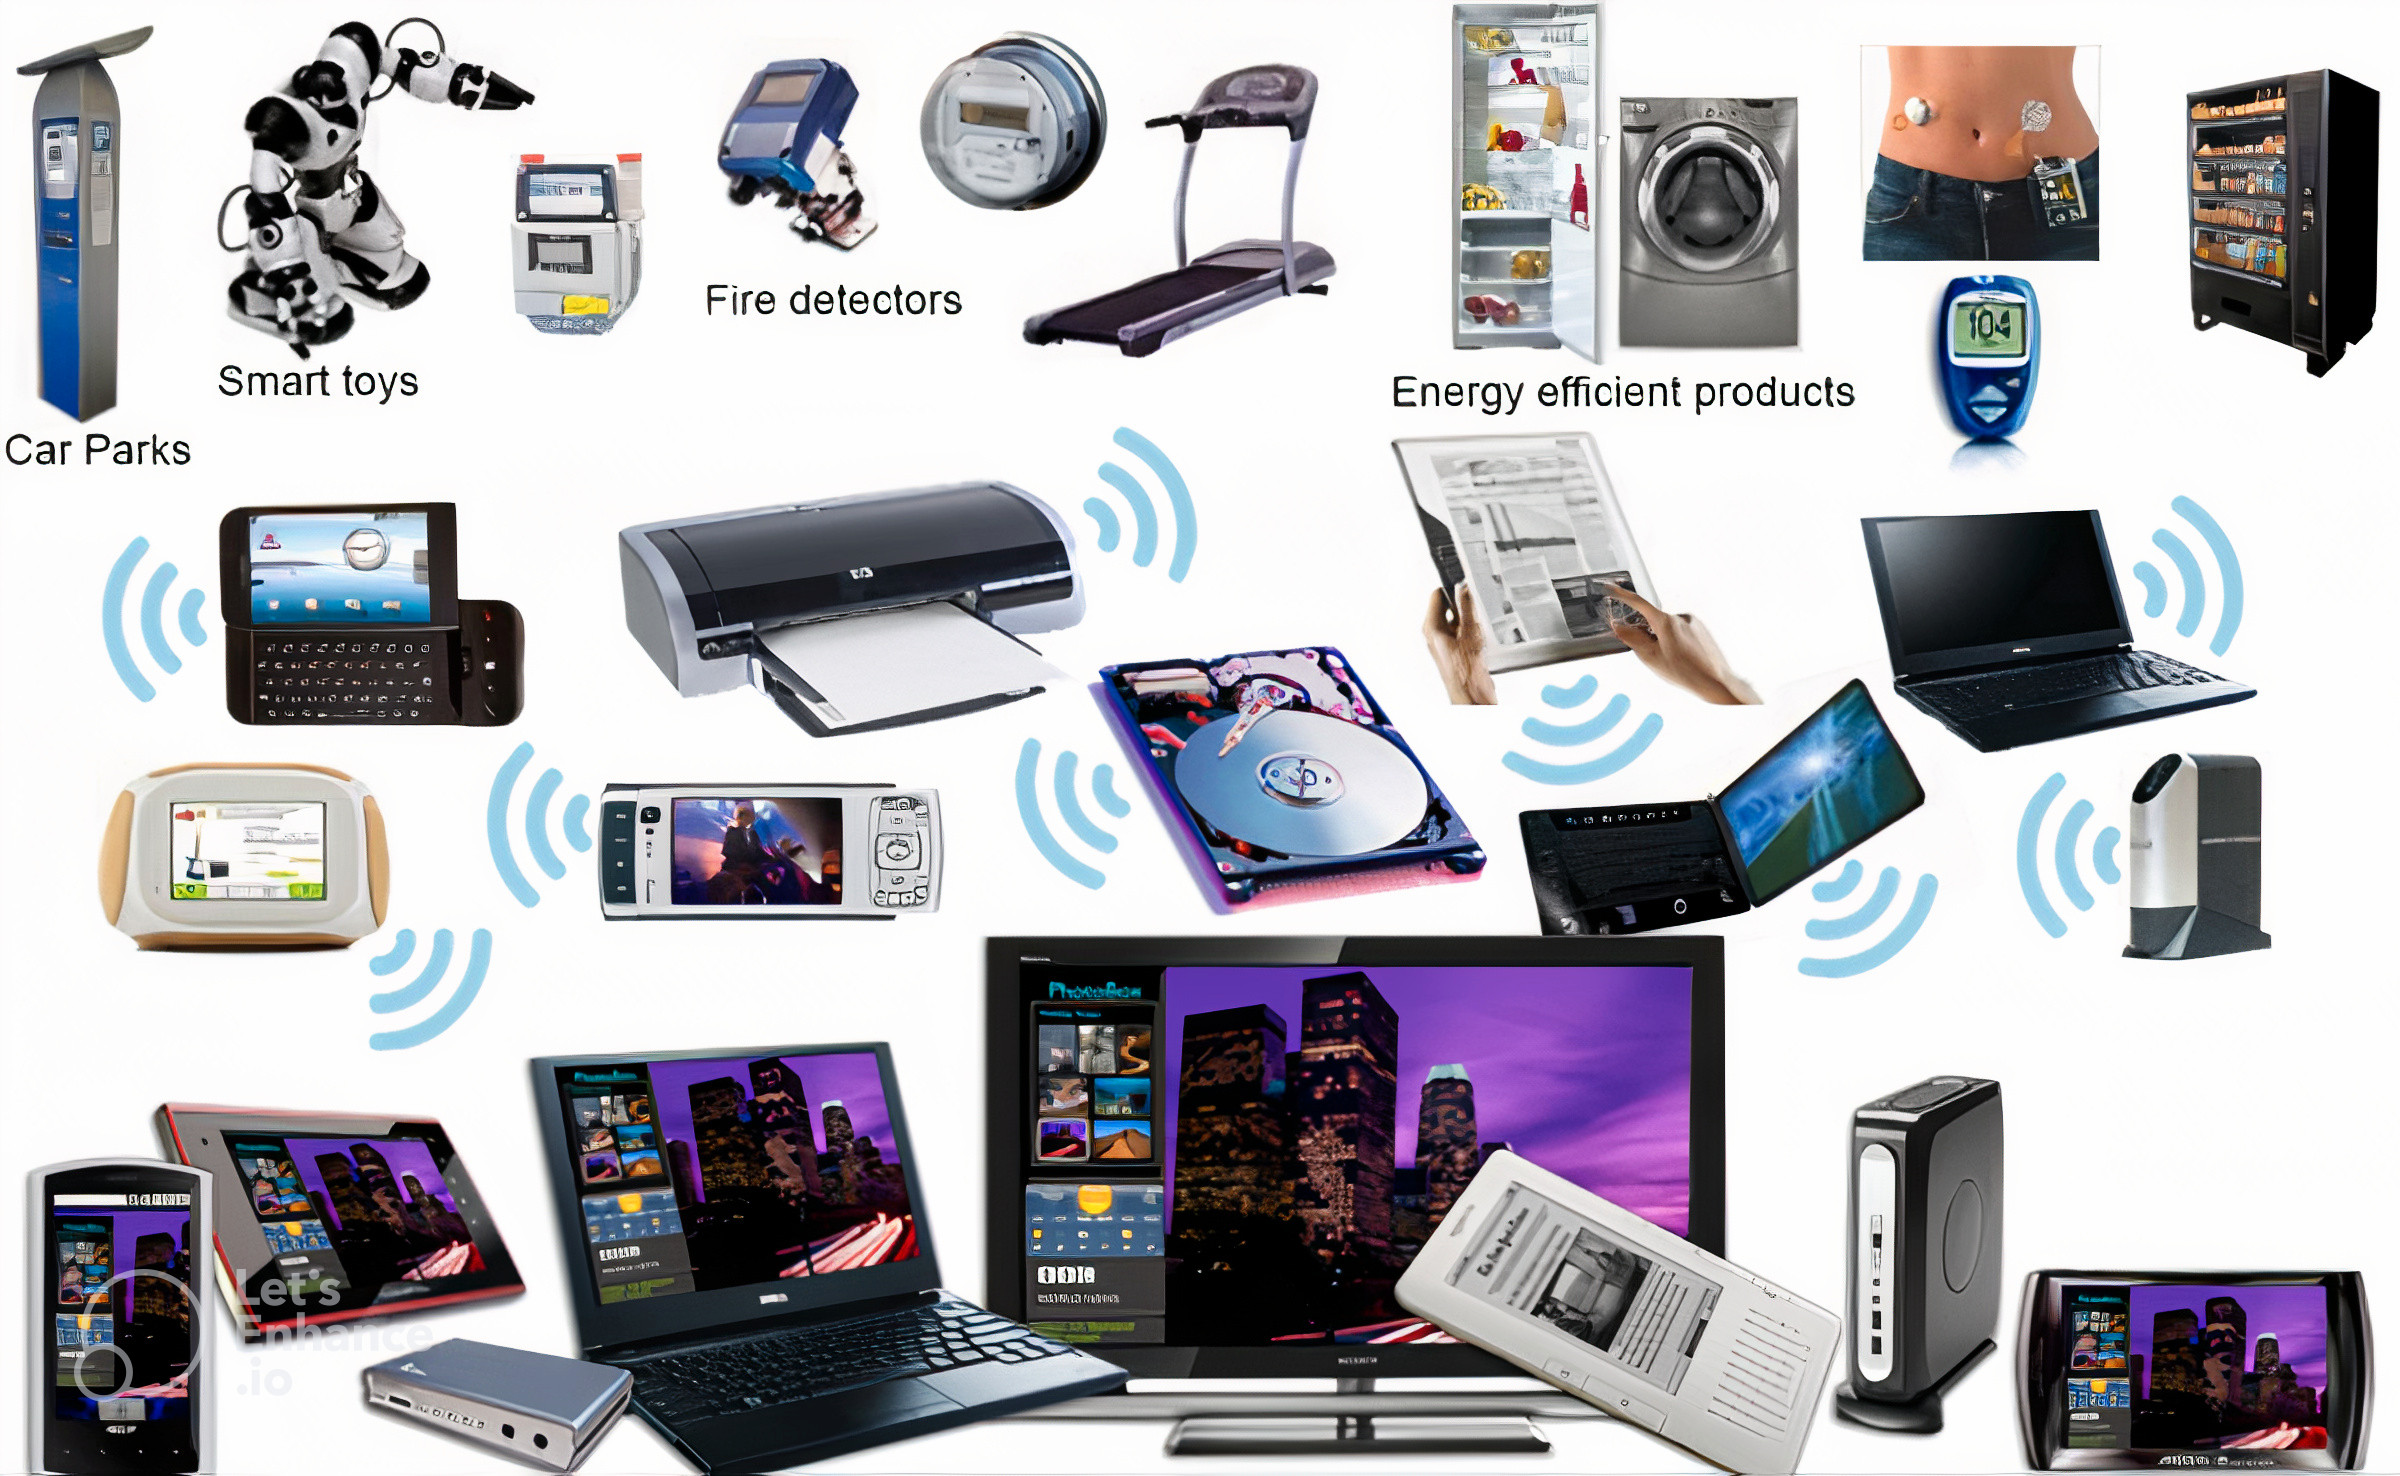
\includegraphics[width=0.85\textwidth]{img/arm_powered_products.jpg}
			\caption{\texttt{ARM} aplikace}
			\label{ARM aplikace}
		\end{figure}
		\column{0.55\textwidth}
			\begin{figure}
			\centering
			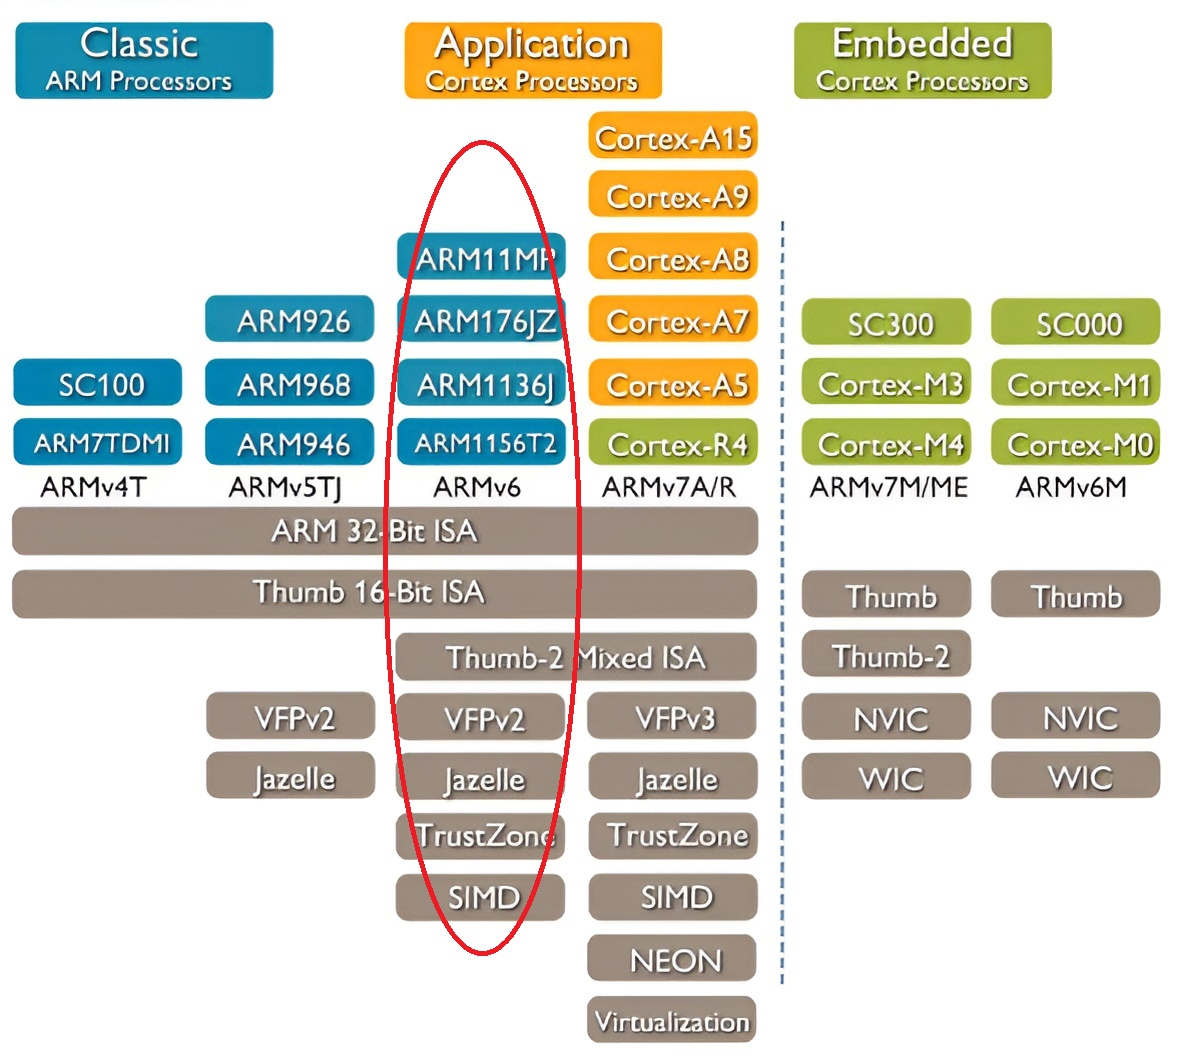
\includegraphics[width=0.9\textwidth]{img/arm_processor_roadmap2.jpeg}
			\caption{\texttt{ARM} \texttt{CPU} roadmap}
			\label{ARM CPU roadmap}
		\end{figure}
	\end{columns}
\end{frame}

\section{Existující řešení}

\subsection{CPUlator}

\begin{frame}
	\vspace{-0.4cm}
	\begin{columns}
		\column{0.5\textwidth}
		\begin{itemize}
			\item \textbf{vhodné pro seznámení se s programování v \texttt{JSA}}
			\begin{itemize}
				\item vizualizace, ladění programu
			\end{itemize}
			\item floating-point instrukce
			\item platformová nezávislost
		\end{itemize}
		\column{0.5\textwidth}
		\begin{figure}
			\centering
			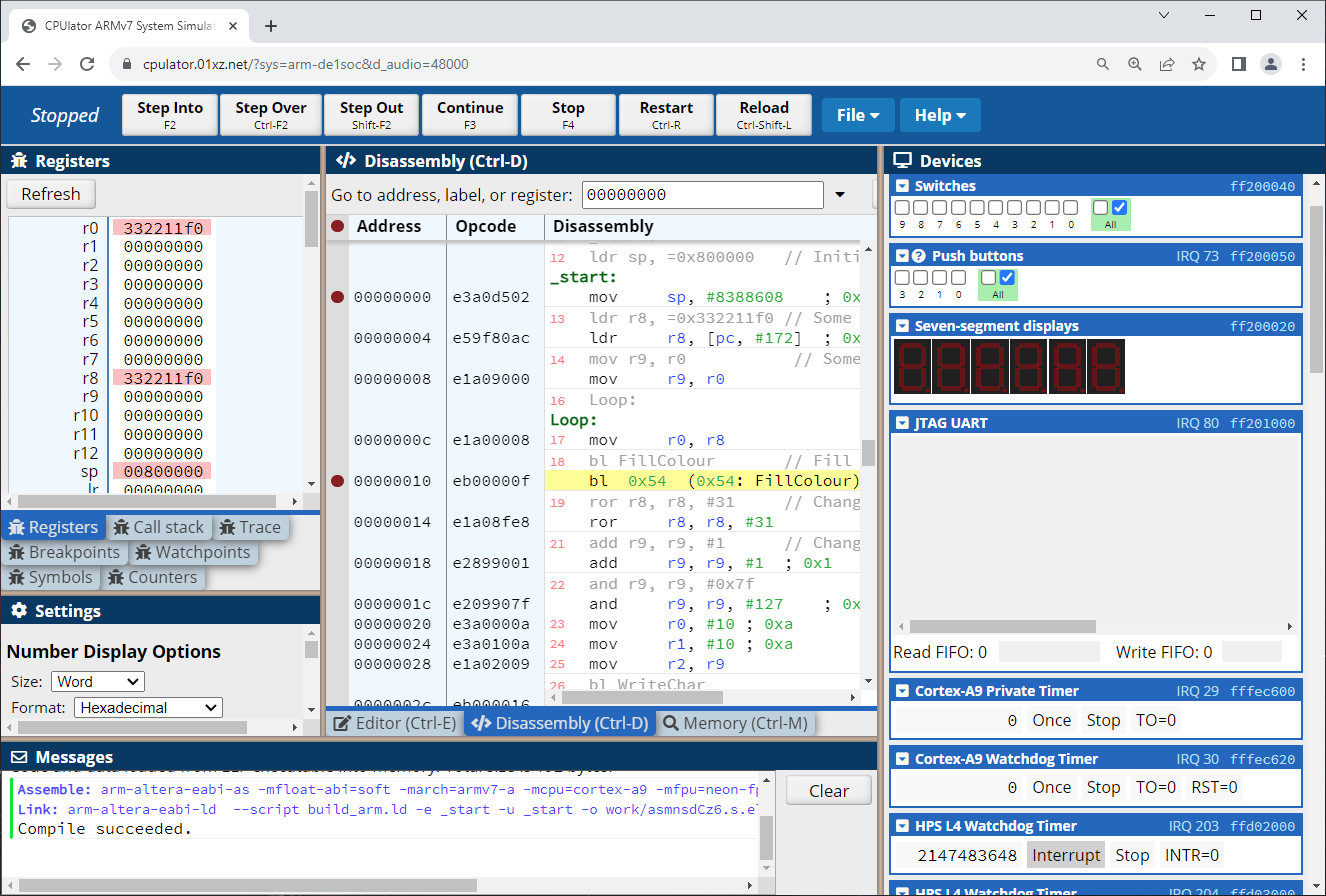
\includegraphics[width=0.85\textwidth]{img/cpulator.png}
			\caption{\href{https://cpulator.01xz.net}{\beamergotobutton{CPUlator}}}
			\label{CPUlator}
		\end{figure}
	\end{columns}
	\noindent\makebox[\linewidth]{\rule{\textwidth}{0.4pt}}
	\begin{block}{Omezení}
		\begin{itemize}
			\item emulace pouze \texttt{CPU} (ne celého \texttt{SoC})
			\item minimální podpora pokročilých systémových operací
			\begin{itemize}
				\item $\Rightarrow$ nevhodné pro testování pricipů \texttt{OS}
			\end{itemize}
			\item limitovaná podpora připojení externích periferií
		\end{itemize}
	\end{block}
\end{frame}

\subsection{QEMU}

\begin{frame}
	\begin{columns}
		\column{0.6\textwidth}
		\begin{itemize}
			\item podpora vícero architektur
			\begin{itemize}
				\item \texttt{x86}, \texttt{MIPS}, \texttt{ARM}, ...
			\end{itemize}
			\item připojení externího debuggeru (\texttt{GNU})
			\item plná podpora systémových operací
		\end{itemize}
		\column{0.4\textwidth}
		\begin{figure}
			\centering
			
\includegraphics[width=0.6\textwidth]{img/Qemu_logo.pdf}
			\caption{\href{https://www.qemu.org}{\beamergotobutton{QEMU}}}
			\label{QEMU}
		\end{figure}
	\end{columns}
	\vspace{0.4cm}
	\noindent\makebox[\linewidth]{\rule{\textwidth}{0.4pt}}
	\begin{block}{Omezení}
		\begin{itemize}
			\item emulace pouze \texttt{CPU} (ne celého \texttt{SoC})
			\item limitovaná podpora připojení externích periferií
			\item \texttt{\_start} symbol očekáván na adrese \texttt{0x00010000} (\texttt{ARM})
			\begin{itemize}
				\item $\Rightarrow$ nekompatibilita s \textit{first-stage} \texttt{BL} \texttt{Rpi0} (\texttt{0x00008000})
			\end{itemize}
			\item problémy se \texttt{systimer}
		\end{itemize}
	\end{block}
\end{frame}

\section{Návrh řešení}

\subsection{ZeroMate - jádro emulátoru (emulovaná funkcionalita)}

\begin{frame}
	\begin{columns}
		\column{0.4\textwidth}
		\begin{block}{\texttt{ARM1176JZF-S}}
			\begin{itemize}
				\item \texttt{ARMv6} instrukce
				\item přepínání režimů \texttt{CPU}
				\item \texttt{ALU}, \texttt{MAC} a \texttt{MMU} (+ \texttt{TLB})
				\item vyjímky a přerušení
				\item podpora ko-procesorů
				\begin{itemize}
					\item \texttt{CP15}, \texttt{CP10}
				\end{itemize}
				\item systémová sběrnice
			\end{itemize}
		\end{block}
		\column{0.4\textwidth}
		\begin{block}{\texttt{BCM2835}}
			\begin{itemize}
				\item \texttt{RAM}
				\item interrupt controller
				\item \texttt{ARM} timer
				\item \texttt{TRNG}
				\item \texttt{GPIO}
				\item \texttt{BSC\_1} (\texttt{I\textsuperscript{2}C})
				\item \texttt{AUX} (\texttt{Mini\_UART})
				\item \textcolor{darkgray}{debug monitor*} 
			\end{itemize}
		\end{block}
	\end{columns}
	\vspace{0.4cm}
	\noindent\makebox[\linewidth]{\rule{\textwidth}{0.4pt}}
	\vspace{-0.4cm}
	\begin{itemize}
		\item \textbf{cílem bylo emulovat nejčastěji používané periferie}
		\item dekompoziční návrh architektury 
		\begin{itemize}
			\item $\Rightarrow$ snadné rozšíření o další periferie
		\end{itemize}
	\end{itemize}
\end{frame}

\subsection{ZeroMate - externí periferie}

\begin{frame}
	\begin{itemize}
		\item jednotné rozhraní pro externí periferie
		\item načtené za běhu jako sdílené knihovny
		\begin{itemize}
			\item možnost načtení vícero instancí (např. \texttt{led.dll})
		\end{itemize}
		\item nezávislé na toolchainu jádra emulátoru
		\begin{itemize}
			\item \texttt{extern "C" \_\_declspec(dllexport)}
		\end{itemize}
	\end{itemize}
	\vspace{0.0cm}
	\begin{figure}
		\centering
		%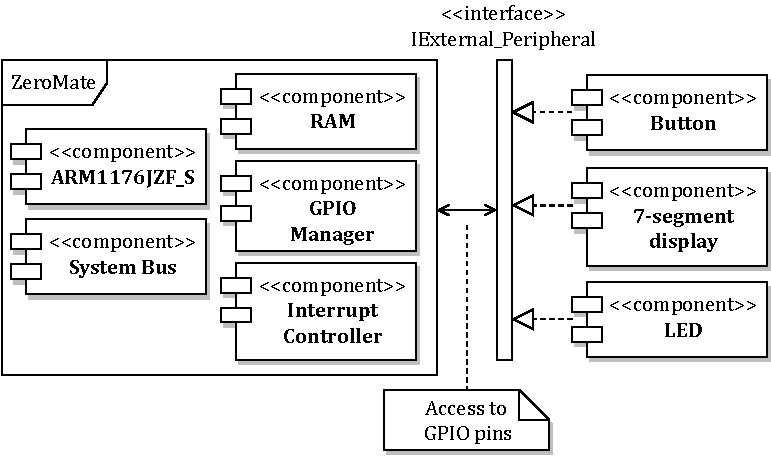
\includegraphics[width=0.58\textwidth]{img/peripheral_interface.pdf}
		\hspace{0.4cm}
		\vspace{-0.4cm}
		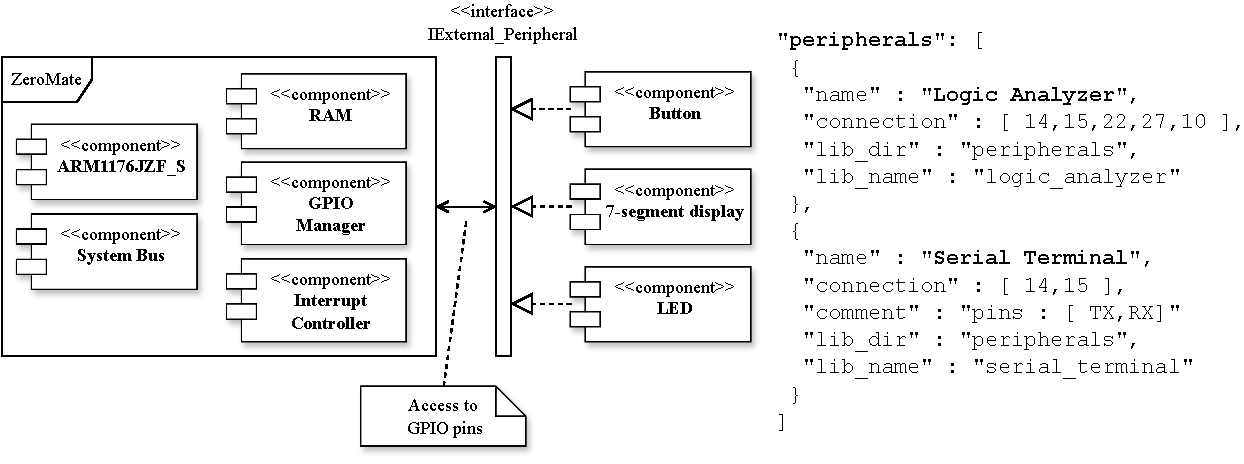
\includegraphics[width=0.92\textwidth]{img/peripheral_interface_3.pdf}
		\vspace{0.2cm}
		\caption{Rozhraní externích periferií}
	\end{figure}
\end{frame}

\section{Ukázka (\texttt{GUI})}

\subsection{ZeroMate - uživatelské rozhraní}

\begin{frame}
	\centering \Large
	\begin{overlayarea}{\textwidth}{\textheight}
		\begin{figure}
			\centering
			\only<1>
			{%
				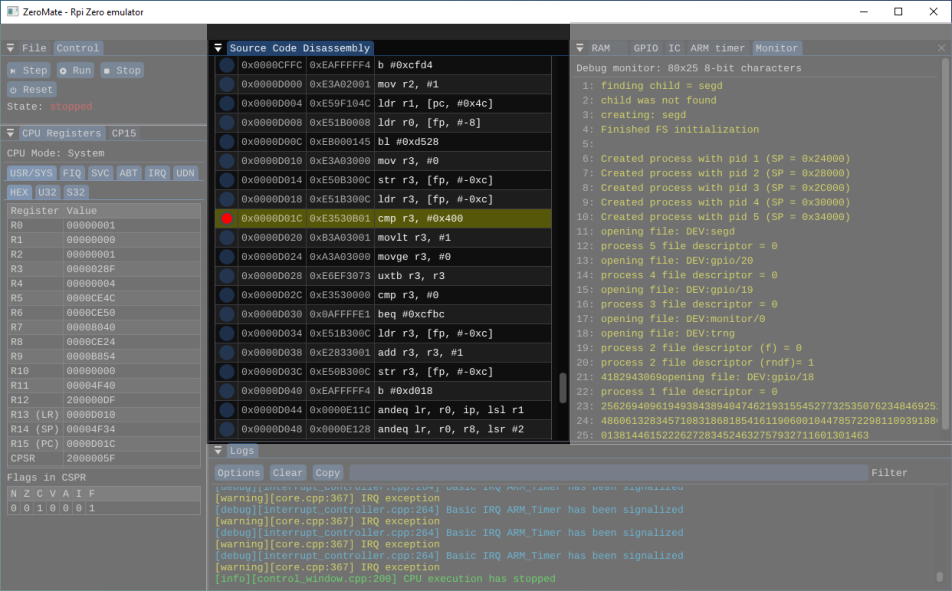
\includegraphics[width=.85\textwidth]{img/gui/01.pdf}%
				\vspace{-0.4cm}
				\caption{a) Disassembly vstupního \texttt{ELF} souboru}
			}%
			\only<2>
			{%
				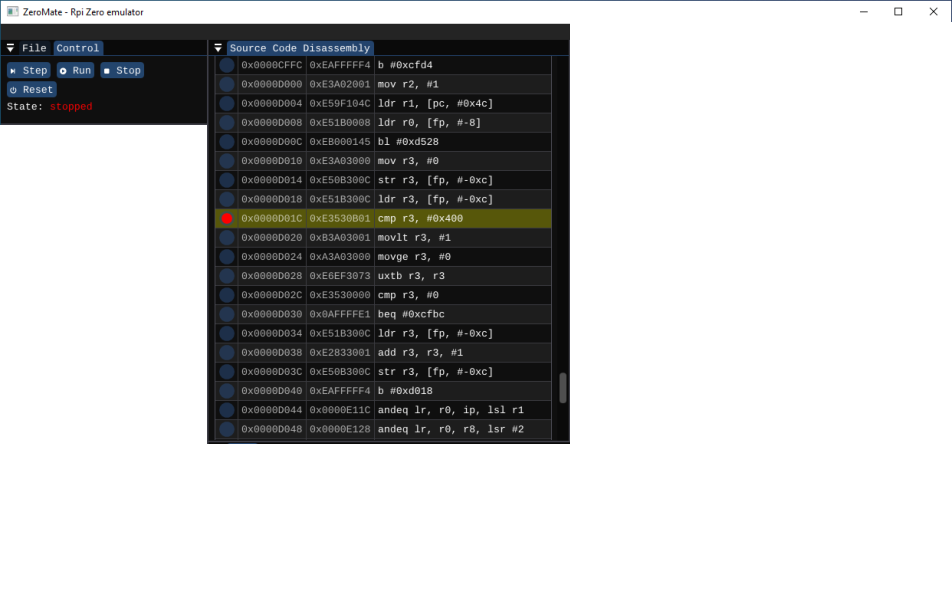
\includegraphics[width=.85\textwidth]{img/gui/02.pdf}%
				\vspace{-0.4cm}
				\caption{b) Řízení emulace (start, stop, step a reset)}
			}%
			\only<3>
			{%
				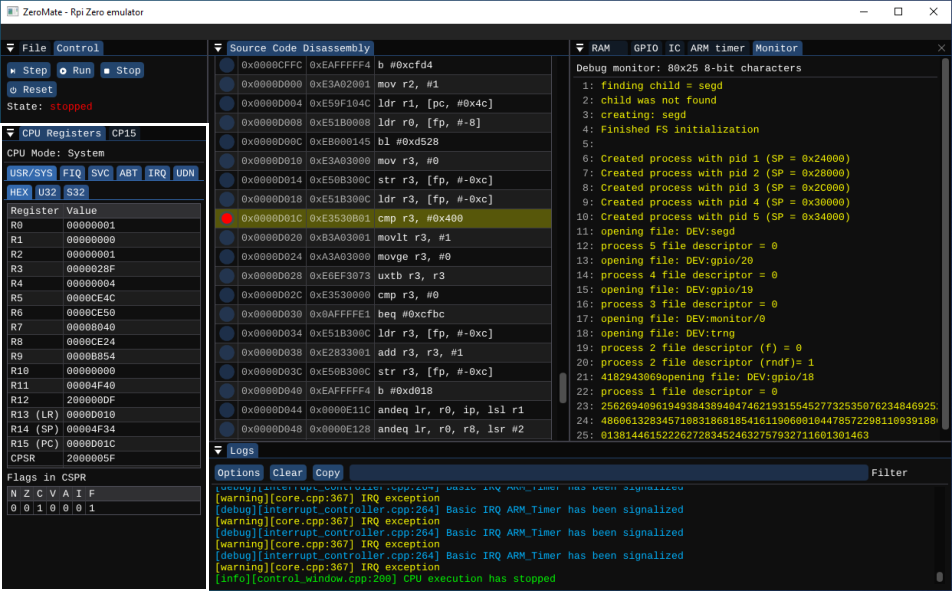
\includegraphics[width=.85\textwidth]{img/gui/03.pdf}%
				\vspace{-0.4cm}
				\caption{c) Registry \texttt{CPU} a systémový koprocesor \texttt{CP15}}
			}%
			\only<4>
			{%
				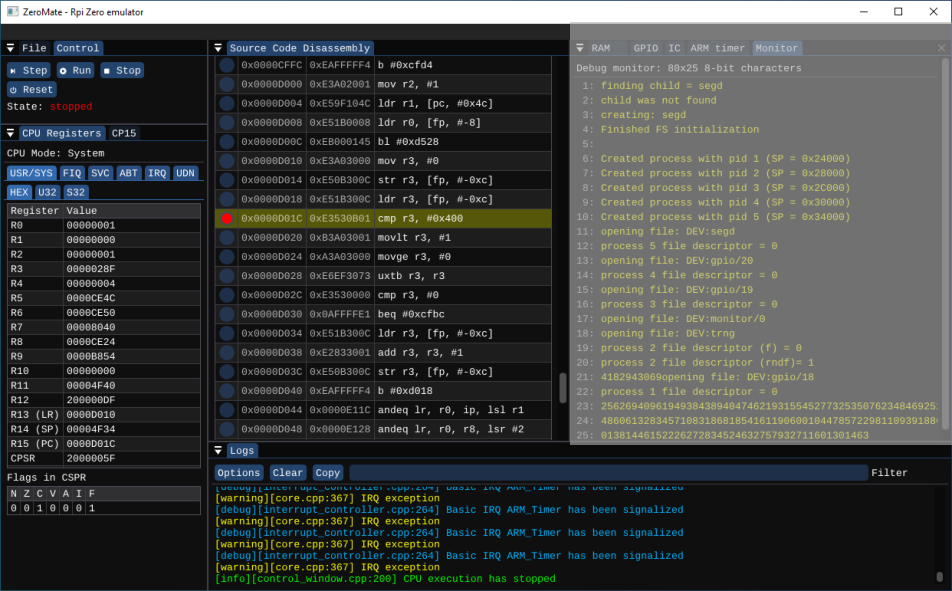
\includegraphics[width=.85\textwidth]{img/gui/04.pdf}%
				\vspace{-0.4cm}
				\caption{d) Logování událostí (přerušení, vyjímky, ...)}
			}%
			\only<5>
			{%
				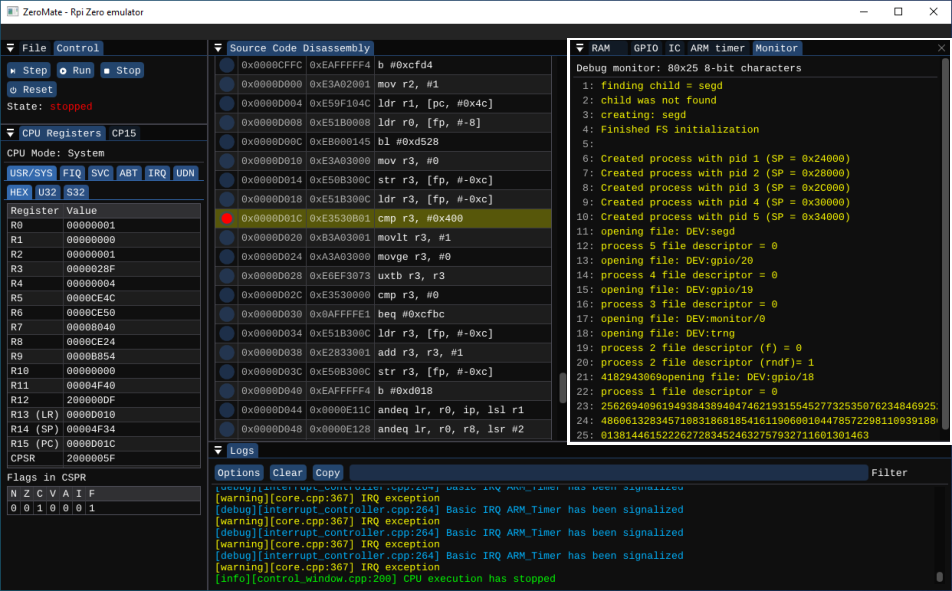
\includegraphics[width=.85\textwidth]{img/gui/05.pdf}%
				\vspace{-0.4cm}
				\caption{e) \texttt{BCM2835} periferie (registry + interpretace hodnot)}
			}%
		\end{figure}
	\end{overlayarea}      
\end{frame}

\subsection{ZeroMate - externí periferie}

\begin{frame}
	\centering \Large
	\begin{overlayarea}{\textwidth}{\textheight}
		\begin{figure}
			\centering
			\only<1>
			{%
				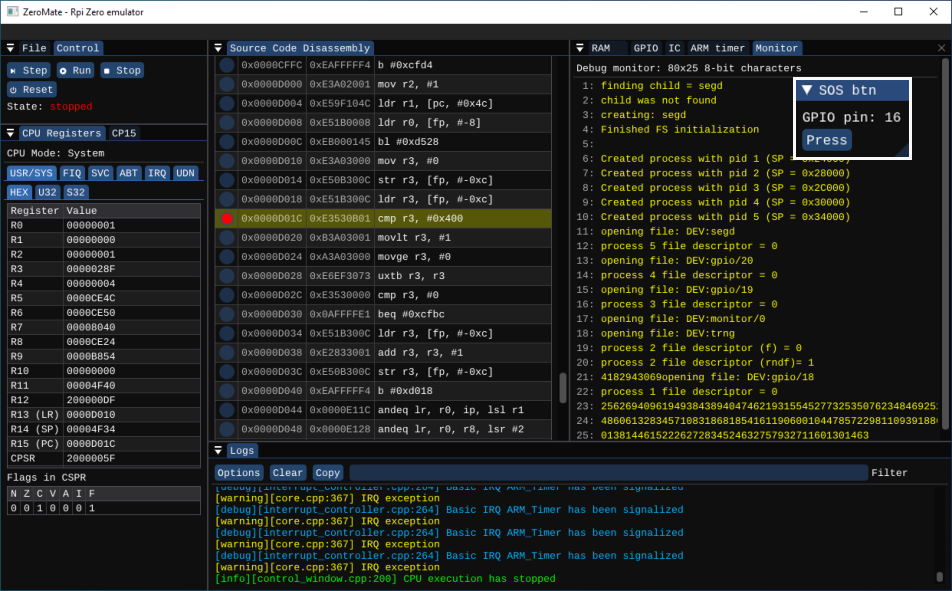
\includegraphics[width=.85\textwidth]{img/screenshot-02.pdf}%
				\vspace{-0.4cm}
				\caption{a) Tlačítko (další periferie viz  \href{https://home.zcu.cz/~ublm/files/os/kiv-dpp-01-en.pdf}{\beamergotobutton{KIV-DPP-01}})}
			}%
			\only<2>
			{%
				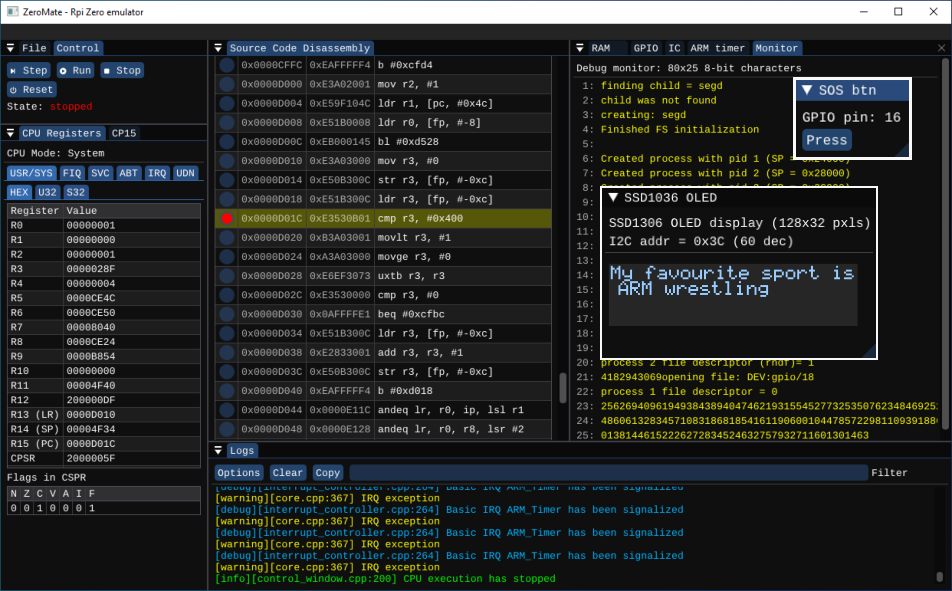
\includegraphics[width=.85\textwidth]{img/screenshot-03.pdf}%
				\vspace{-0.4cm}
				\caption{b) \texttt{SSD1036} \texttt{OLED} displej řízený přes \texttt{I\textsuperscript{2}C}}
			}%
			\only<3>
			{%
				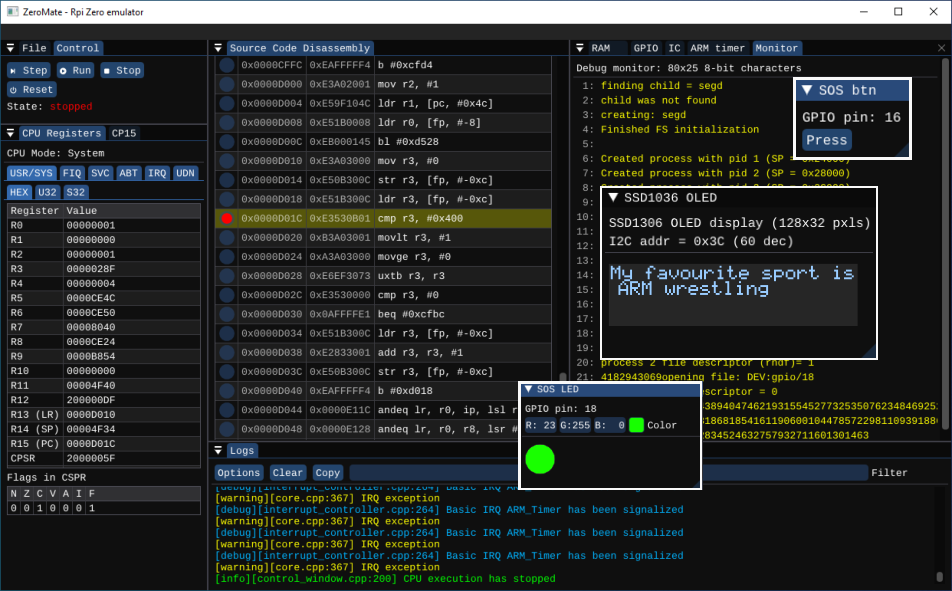
\includegraphics[width=.85\textwidth]{img/screenshot-04.pdf}%
				\vspace{-0.4cm}
				\caption{c) \texttt{RGB} \texttt{LED}}
			}%
			\only<4>
			{%
				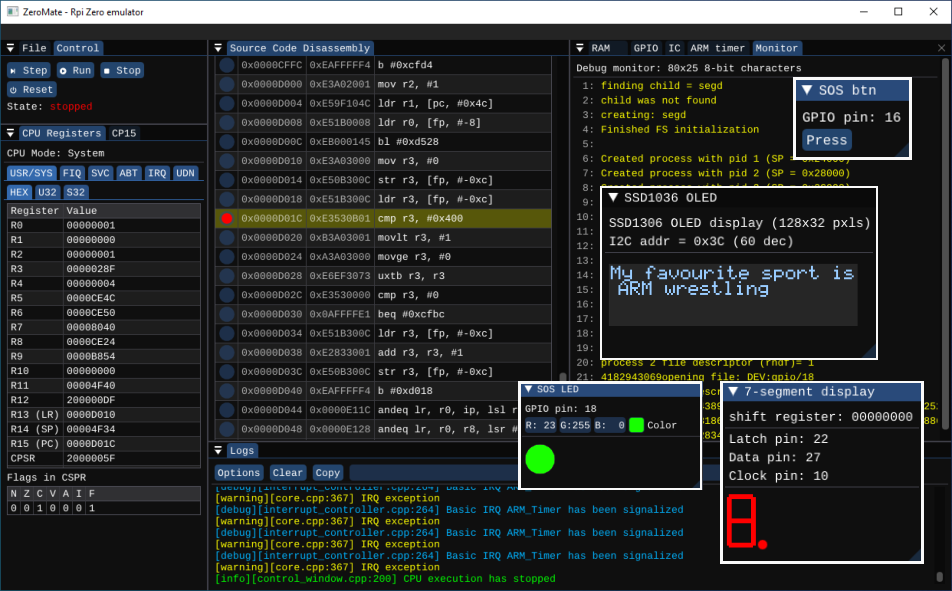
\includegraphics[width=.85\textwidth]{img/screenshot-05.pdf}%
				\vspace{-0.4cm}
				\caption{d) Sedmisegmentový \texttt{LED} displej řízený posuvným registrem}
			}%
			\only<5>
			{%
				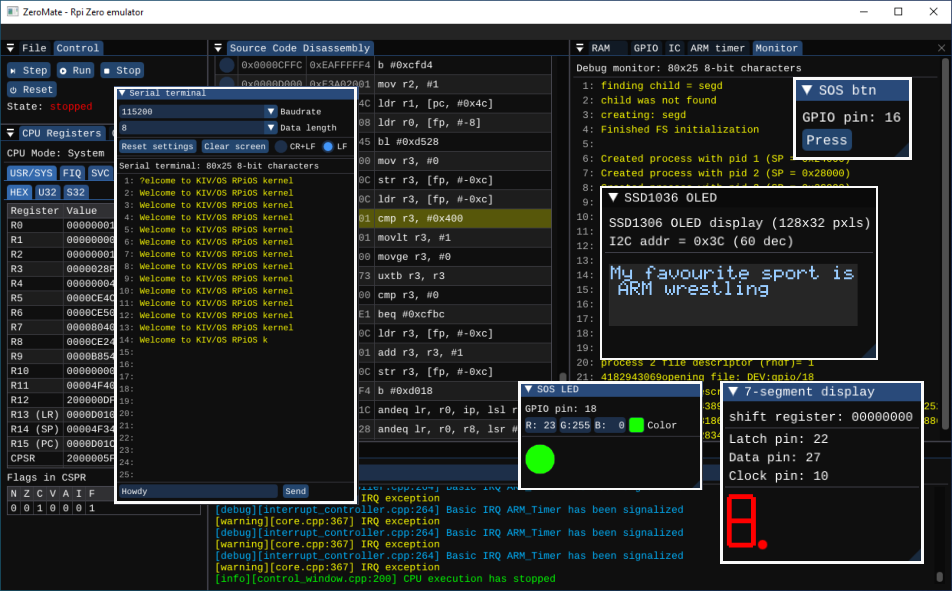
\includegraphics[width=.85\textwidth]{img/screenshot-06.pdf}%
				\vspace{-0.4cm}
				\caption{e) Sériový terminál (\texttt{UART})}
			}%
			\only<6>
			{%
				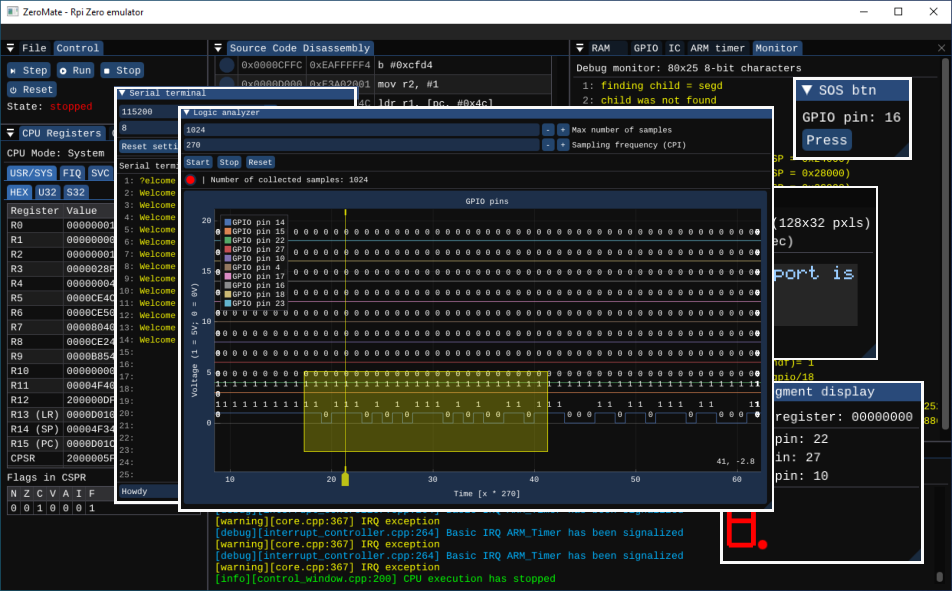
\includegraphics[width=.85\textwidth]{img/screenshot-07.pdf}%
				\vspace{-0.4cm}
				\caption{f) Logický analyzátor}
			}%
		\end{figure}
	\end{overlayarea}
\end{frame}

\section{Technlogie}

\subsection{Vývoj a pouižité technologie}

\begin{frame}
	\vspace{-0.5cm}
	\begin{figure}
		\centering
		
\includegraphics[width=0.07\textwidth]{img/logos/github.pdf}
	\end{figure}
	\centering
	\vspace{-0.4cm}
	\href{https://github.com/silhavyj/ZeroMate}{\beamergotobutton{https://github.com/silhavyj/ZeroMate}}
	\vspace{-0.1cm}
	\noindent\makebox[\linewidth]{\rule{\textwidth}{0.4pt}}
	\begin{columns}
		\column{0.5\textwidth}
		\begin{block}{vývoj}
			\begin{itemize}
				\item \texttt{C++20} (\texttt{Clang}, \texttt{GCC} a \texttt{MSVC})
				\item \texttt{CMake}
				\item Linux, Windows, \textcolor{darkgray}{MacOS*}
			\end{itemize}
		\end{block}
		\column{0.4\textwidth}
		\begin{block}{\texttt{CI} pipeline}
			\begin{itemize}
				\item \href{https://app.codecov.io/gh/silhavyj/ZeroMate}{\beamergotobutton{Codecov}}
				\item \href{https://app.codacy.com/gh/silhavyj/ZeroMate/dashboard}{\beamergotobutton{Codacy}}
				\item \href{https://silhavyj.github.io/ZeroMate}{\beamergotobutton{Doxygen}}
			\end{itemize}
		\end{block}
	\end{columns}
	\vspace{0.2cm}
	\noindent\makebox[\linewidth]{\rule{\textwidth}{0.4pt}}
	\vspace{-0.3cm}
	\begin{itemize}
		\item knihovny třetích stran automaticky staženy a sestaveny \\ (\texttt{.gitmodules} + \texttt{CMake})
		\begin{itemize}
			\item \href{https://github.com/google/googletest}{\beamergotobutton{GoogleTest}} \href{https://github.com/ocornut/imgui}{\beamergotobutton{ImGUI}}
			\href{https://github.com/martin-olivier/dylib}{\beamergotobutton{dylib}} 
			\href{https://github.com/serge1/ELFIO}{\beamergotobutton{ELFIO}} 
			\href{https://github.com/glfw/glfw}{\beamergotobutton{GLFW}} 
			\href{https://github.com/capstone-engine/capstone}{\beamergotobutton{capstone}}
		\end{itemize}
	\end{itemize}
\end{frame}

\section{Testování}

\subsection{Funkcionalita emulátoru}

\begin{frame}
	\begin{block}{1) Unit testy}
		\begin{itemize}
			\item jádro emulátoru (exekuce \texttt{ARMv6} instrukcí)
			\item GoogleTest, \texttt{CI} (regresní testy), \textbf{pokrytí $\approx$ 78\%}
		\end{itemize}
	\end{block}
	\begin{block}{2) Funkční testy}
		\begin{itemize}
			\item \texttt{BCM2835} periferie
			\item připravená sada příkladů (\texttt{.ELF})
			\begin{itemize}
				\item \texttt{UART}, \texttt{FPU}, \texttt{GPIO}, \texttt{I\textsuperscript{2}C}, plánování procesů (\texttt{EDF}, \texttt{RTL}), \texttt{ARM} timer, ...
				\item \textbf{součástí repozitáře jako examples}
			\end{itemize}
		\end{itemize}
	\end{block}
	\begin{block}{3) Aplikační testy, \texttt{GUI}}
		\begin{itemize}
			\item \texttt{KIV/OS} cvičení
			\item dotazník hodnocení celkové použitelnosti
		\end{itemize}
	\end{block}
\end{frame}

\subsection{Výkonnost emulace \texttt{ARMv6} instrukcí}

\begin{frame}
	\begin{itemize}
		\item \textbf{výkon emulátoru $\approx$ 4-5 Minst/s} (\href{https://github.com/MartinUbl/KIV-RTOS}{\beamergotobutton{KIV-RTOS}})
		\item analýza rychlosti emulace jednotlivých instrukcí
		\begin{itemize}
			\item $\Rightarrow$ potenciální optimalizace
		\end{itemize}
	\end{itemize}
	\begin{figure}
		\centering
		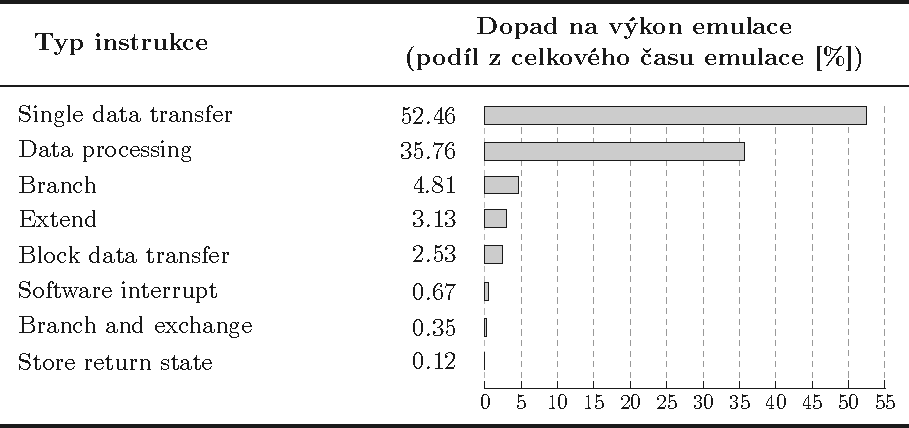
\includegraphics[width=0.8\textwidth]{img/performance_2_cz.pdf}
	\end{figure}
	\footnote{\tiny Měřeno na: \textit{Lenovo ThinkPad P50 laptop; Windows 10; \newline Intel(R) Core(TM) i7-6820HQ; \texttt{2.70GHz}; \texttt{16GB}} \vspace{0.5cm}}
\end{frame}

\subsection{Porovnání výkonnosti s ostatními emulátory}

\begin{frame}
	\vspace{-0.2cm}
	\begin{figure}
		\centering
		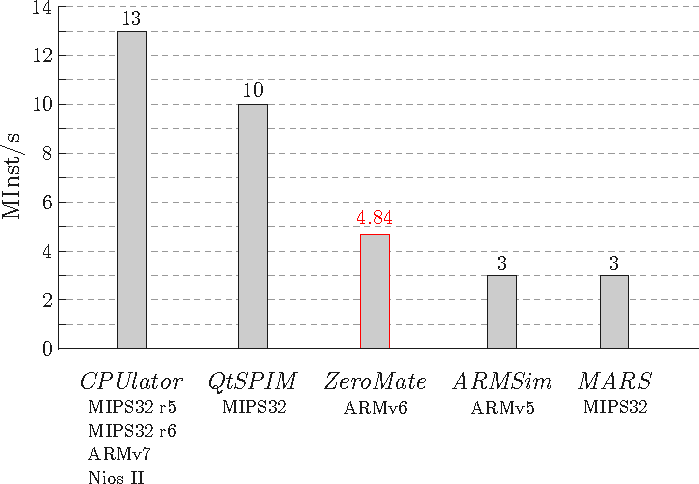
\includegraphics[width=0.62\textwidth]{img/performance_comparison.pdf}
	\end{figure}
	\vspace{-0.4cm}
	\noindent\makebox[\linewidth]{\rule{\textwidth}{0.4pt}}
	\vspace{-0.4cm}
	\begin{itemize}
		\item \textbf{pouze orientační} (\href{https://cpulator.01xz.net/}{\beamergotobutton{https://cpulator.01xz.net [2023]}})
		\item \textbf{ZeroMate jako jediný podporuje \texttt{MMU}}
		\begin{itemize}
			\item využití s každým přístupem do paměti ($\approx$ 42\% instrukcí)
		\end{itemize}
	\end{itemize}
\end{frame}

\section{Závěr}

\subsection{Návrhy na budoucí vylepšení}

\begin{frame}
	\begin{block}{\texttt{IPC}}
		\begin{itemize}
			\item např. pomocí socketů
			\item spuštění vícero instancí ZeroMate emulátoru
			\begin{itemize}
				\item $\Rightarrow$ emulace distribuovaných systémů \& algoritmů
			\end{itemize}
		\end{itemize}
	\end{block}
	\begin{block}{\texttt{CLI} mód}
		\begin{itemize}
			\item integrace do \texttt{CI/CD} pipeline
			\item validace programů v rámci výuky
			\begin{itemize}
				\item např. definováním očekáváné \texttt{UART} komunikace (\texttt{I/O})
			\end{itemize}
		\end{itemize}
	\end{block}
	\noindent\makebox[\linewidth]{\rule{\textwidth}{0.4pt}}
	Další viz text \href{https://github.com/silhavyj/ZeroMate/blob/main/docs/latex/DP_silhavyj_A21N0072P.pdf}{\beamergotobutton{diplomové práce}}...
\end{frame}

\begin{frame}
  \centering \Large
  Děkuji Vám za pozornost\\
  \href{https://github.com/silhavyj/ZeroMate}{\beamergotobutton{https://github.com/silhavyj/ZeroMate}}
  \begin{figure}
  	\centering
  	
\includegraphics[width=0.10\textwidth]{img/qr-code.pdf}
  \end{figure}
\end{frame}

\appendix

\section{Otázky}

\subsection{Otázka 1}

\begin{frame}
	\begin{block}{Otázka}
	\end{block}
	\begin{block}{Odpověď}
	\end{block}
\end{frame}

\subsection{Otázka 2}

\begin{frame}
	\begin{block}{Otázka}
	\end{block}
	\begin{block}{Odpověď}
	\end{block}
\end{frame}



\end{document}